% This is a LaTeX template for poster using University of Helsinki style
% This version uses pdflatex; if you have XeTeX available, 
% consider using poster_xetex.tex for fancy font settings
%
% The official Graphical Instructions available from hy.logodomain.com (from university network only) defines colours, fonts etc. This Template does not perfectly match the official poster template of the university
%
% Jukka Suomela's collection of LaTeX tricks has been invaluable in building this template: http://cs.helsinki.fi/u/josuomel/latex/ 
%
% Original template by Janne Korhonen
% This file by Juha Karkkainen

% Encoding of this file is iso-8859-1 latin 1

\documentclass[a4paper]{article} % This actually makes poster of size A4, scale up when printing. Used text font size is a bit small for A1 poster, preferably use \small in that case 


% Misc. packages
\usepackage[T1]{fontenc}
\usepackage{url}
\usepackage{amsfonts}
\usepackage[font=small]{caption}
\usepackage[english]{babel}
\usepackage[absolute]{textpos}
\usepackage{amssymb}
\usepackage{amsmath} 
\usepackage{amsthm}

% Graphics stuff
\usepackage[usenames,dvipsnames]{color}
\usepackage{graphicx}

% algorithm stuff
\usepackage{float}
\usepackage{subfigure}
\usepackage{algpseudocode}
\usepackage{algorithm}


% My favourite macros
\newcommand{\N}{\mathbb{N}} %natural numbers
\newcommand{\Z}{\mathbb{Z}} %integers
\newcommand{\Q}{\mathbb{Q}} %rationals
\newcommand{\R}{\mathbb{R}} %reals

\newcommand{\G}{\mathcal{G}} % fancy G
\newcommand{\A}{\mathcal{A}} % fancy A
\newcommand{\bO}{\mathcal{O}} % fancy O

\newcommand{\eos}{\#}
\newcommand{\rank}{\textsc{rank}}


% enumitem for controlling enumerate and itemize environments; usefull for saving space
\usepackage{enumitem}


% Fonts
%
% Palantino - Helvetica - Courier.
% I haven't really spent time to figure out how to best match the official university style with latex font packages, as I use XeTex myself...
\usepackage{mathpazo}
\linespread{1.10}
\usepackage[scaled]{helvet}
\usepackage{courier}

% Colours
\definecolor{sciorange}{RGB}{252,163,17}
\definecolor{unigray}{RGB}{140,140,140}
\definecolor{first}{RGB}{180,30,10}
\definecolor{second}{RGB}{10,120,130}
\definecolor{new}{RGB}{190,50,10}
\definecolor{wavelet}{RGB}{70,140,220}
%\definecolor{improved}{RGB}{80,200,80}
\definecolor{improved}{RGB}{10,100,160}
\definecolor{prior}{RGB}{140,140,140}

% Textpos to manually position blocks of text on the page
\usepackage[absolute]{textpos}

% We define 1 mm grid for positioning the text blocks on the page
% The idea is to leave 10 mm marginals to all sides; the three text columns are 60 mm wide with 5 mm space between columns.
\setlength{\TPHorizModule}{1mm}
\setlength{\TPVertModule}{1mm}

% The origin is set to right below the main title; this means that main title blocks have negative y-coordinate. There is actually no good reason for this, I just happened to do this that way.
\textblockorigin{10mm}{48.5mm}


% parindent is set to zero, because it looks better in posters
% you could also add some space between paragraphs here, but I use manual vertical spaces in this sample
\setlength{\parindent}{0pt}


% Finally, the content
\begin{document}
\pagestyle{empty} % To get rid of page numbers and so


% ------------------------------------------------------------------------------------------------------------------------------
% Main title, University logo etc.

% If you need more space for the title or want the logo to be bigger, you need to adjust various parameters, as I did not bother to automate this yet
% Mainly, move the textblockorigin above down and adjust all the boxes here to be higher up.

% First, the University logo. The included flame.pdf is a copy of the official logo in vector format, so it is good for all sizes.
% Box starts 10 mm from the top
\begin{textblock}{95}(0,-38.5)

\includegraphics[width=22mm]{flame}
\end{textblock}	

% University - Faculty - Department
% Box starts 10 mm from the top
\begin{textblock}{95}(95,-38.5)
{\fontsize{8}{7}\selectfont\sffamily\color{unigray}
\hfill HELSINGIN YLIOPISTO

\hfill HELSINGFORS UNIVERSITET

\hfill UNIVERSITY OF HELSINKI

\color{sciorange}\hfill MATEMAATTIS-LUONNONTIETEELLINEN TIEDEKUNTA

\hfill MATEMATISK-NATURVETENSKAPLIGA FAKULTETEN

\hfill FACULTY OF SCIENCE % For some reason, the last line here gets messed up without extra spaces...


}
\end{textblock}


% Main title
% If you need two lines for the title, you need to adjust the position of this block and textblockorigin
% Remember, two first words use faculty colour. If your title is long, you can use small letters.
\begin{textblock}{190}(0,-13.5)
{\sffamily\LARGE{{\color{sciorange}AHO-CORASICK \color{unigray}AND RABIN-KARP IN MULTIPLE PATTERN\\ STRING MATCHING}}}
\small\hfill Aleksi Hartikainen and Jussi Kokkala\\ % If you have multiple authors, their names can be on the same line. Adjust font size as necessary
\rule[2mm]{190mm}{0.3pt} % This is the line under the title, adjust the last parameter if it seems to be in the wrong place
\end{textblock}

% ------------------------- ABSTRACT ----------------------------------
% The "abstract" block. Does not actually exist in the university poster template, so you may consider not using this
\begin{textblock}{92.5}(0,0)
\sffamily
\small 
The Burrows-Wheeler transform (BWT) is a powerful tool for data
compression used for example in the popular compression program
bzip2. The \emph{inverse} BWT is usually the bottleneck in the
decompression phase with respect to both space and time.
\end{textblock}
\begin{textblock}{92.5}(97.5,0) 
  \sffamily \small 
  Our new algorithms improve the performance of inverse BWT.  They
  range from the fastest known algorithm to the most space-efficient
  one, and cover the whole space-time tradeoff spectrum in between.
\end{textblock}

 %Large subtitle with line. Again, not from the university template.
\begin{textblock}{190}(0,25)
\sffamily
\Large{\color{sciorange}ALGORITHMS}\small\\
\rule[3mm]{190mm}{0.1pt}
\end{textblock} 

% ---------------------------- INTRO ----------------------------------
% Three-column stuff
%
% The vertical size of the columns depends on the content, so unfortunately you have to manually move contents around

% First column
\begin{textblock}{60}(0,32)
  {\sffamily\normalsize{\color{sciorange}AHO--CORASICK
      }}\vspace{1mm}\\ % Titles among the main text are made like this, not by using \section
\footnotesize 

Aho-Corasick matching algorithm constructs an automaton (Figure \ref{fig:ac_machine}) which is then computed on the text.
Dotted links in figure \ref{fig:ac_machine} are followed until matching transition is found. From the $\bot$ state there is transition
to starting state with all symbols.

%Running time of the algorithm is linear in the length of text. Each failure link goes towards the root, so in total we can't use more failure
%links than we do transitions.

First we create a trie of all pattern strings. Then we traverse the trie in breadth first order.

% Use includegraphics with width same as the current block width
%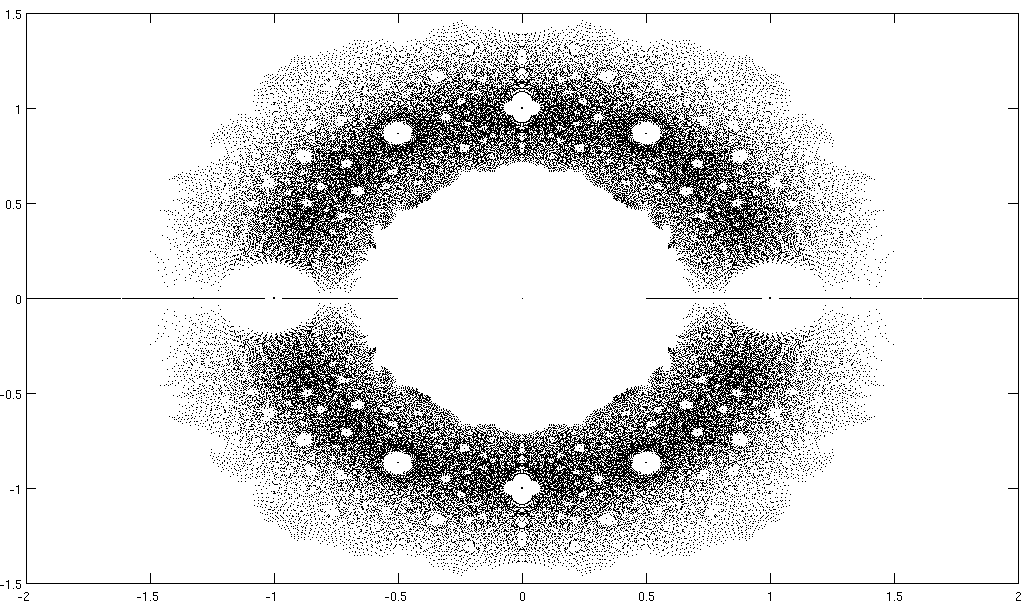
\includegraphics[width=60mm]{zeros.png}

% Captions are in sans-serif font, with smaller typeface than the main text.
%\scriptsize\sffamily Complex zero points of polynomials with degree at most $8$ and coefficients in $\{ -1, 0, 1\}$.

\vspace{5mm}

\begin{algorithm} 
\label{ac_fail}
\caption{Algorithm for computing failure links}

\begin{algorithmic}[1]
\end{algorithmic}
\end{algorithm}

%\Require{Trie of patterns}
%\Ensure{Failure links for all states}
%\State  fail[root]$ \gets \bot$
%\State enqueue(root)
%\While {queue is not empty}
%\State $v \gets $ dequeue()
%\EndWhile

%    v = dequeue()
%while (queue is not empty)
%    for each transition (u, s):
%        w = fail[v]
%        while (trie[w][s]==null))
%            w = fail[v]
%        fail[u] = transition[w][s]
%        enqueue(u)
%

\begin{figure}
\label{fig:ac_machine}
\centering
 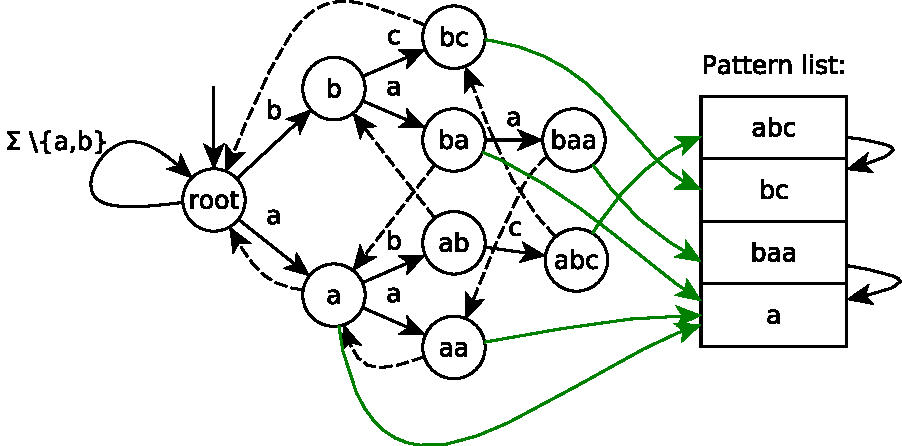
\includegraphics[width=60mm]{aho_corasick.eps}
\caption{Aho-Corasick automaton with failure links and pattern links}
\end{figure}


%During the construction of the automaton we also create pattern links, which link each pattern $s_i$ to
%longest pattern 
%For each accepting state there is a link to the longest matching pattern in patter
%
%In addition to the automaton Aho-Corasick algorithm creates linked 
%For each matching state we have a link to 


\end{textblock} 

% Second column
\begin{textblock}{60}(65,32)
  {\sffamily\normalsize{\color{sciorange}RABIN--KARP}}\vspace{1mm}\\
  \footnotesize 
      Rabin-Karp uses hashing to find fixed length patterns in a text. The hashing function used is a rolling hash, meaning that the hash of $T[2\;..\;N+1]$ can be calculated from the hash of $T[1..N]$ in constant time. 
     
If the hash values of $T[i\;..\;N+i]$ and a pattern prefix of length N, the algorithm checks if the pattern occurs at text index $i$.

    For $P$ patterns of combined length $m$  and a text of length $n$, the average running time of Rabin-Karp is $O(n+m)$ in space $O(P)$.
\end{textblock}


% ----------------------- EXPERIMENTS ----------------------------

\begin{textblock}{190}(0,120)
\sffamily
\Large{\color{sciorange}EXPERIMENTAL RESULTS}\small\\
\rule[3mm]{190mm}{0.1pt}
\end{textblock} 


\begin{textblock}{60}(0,125) 
\end{textblock}

\begin{textblock}{60}(65,125) 
\end{textblock} 


%\begin{textblock}{60}(130,165)
%  {\sffamily\normalsize{\color{sciorange}CONCLUDING REMARKS}}\vspace{1mm}\\
%  \footnotesize 
%\end{textblock}

\begin{textblock}{60}(130,185)
  \def\refname{\normalfont\sffamily\normalsize{\color{sciorange}REFERENCES}}
  \scriptsize\sffamily
  \bibliographystyle{abbrv}
  \bibliography{bib}
\end{textblock}

% Unfortunately, this template has no references. The official instructions seem to indicate that sans-serif font is used for the reference list.

\end{document}
